\documentclass[output=paper]{langscibook} 
\author{Judith Kaplan\affiliation{University of Pennsylvania}}
\title{Visual formalisms in comparative-historical linguistics}
\label{chap:kaplan}


\abstract{This paper examines visual formalisms in comparative-historical linguistics from the perspective of the history of science. It shows that visual aids representing key understandings of language relationship have followed on pre-existing visual metaphors. Using this observation to pry open canonical metaphors of language  relationship, it traces the ways in which these ``visualizations'' have both consolidated existing research programs and opened up new lines of inquiry for students and recent advocates of phylogenetic methods.}

\begin{document}

\maketitle

\section{Introduction}
\label{sec:kaplan:intro}

From the interiority of brain atlases to the distant topography of Mars, from the intimate realm of nano-images to the global modelling of climate data, a recent swell in  computerized visualization techniques is transforming the face of scientific research, pedagogy, and generalist publications. Commenting on this trend in 2014, Lorraine Daston judged computer simulations to be ``the greatest revolution in scientific empiricism since the canonization of observation and experiment in the late seventeenth century'' \citep[321]{Daston2014}. These developments, moreover, have had a profound impact on scholarship in Science and Technology Studies: many have hailed the growing sophistication of digital visual culture as an opportunity to re-think classical theories of scientific representation. Crucially, their efforts have emphasized the \emph{materiality} of scientific representation in a turn away from questions of truth-as-correspondence and social infrastructure. For this new generation, the ``material enactments'' of scientific images are to be taken just as seriously as the embodied practices and community norms surrounding them, and a good deal more seriously than any quest to faithfully represent the natural world (\citealt[3]{Coopmansetal2014}; see also \citealt{Kusukawa2016}).

How might these conversations relate to the formalisms of comparative-historical linguistics?\footnote{See James McElvenny's preface to this volume. This chapter takes formalisms to be those ``devices employed in the representation and analysis of phenomena'' (p. \pageref{p:pref:devices}), as he elaborates.} Like economics, chemistry, and molecular biology, to name a few arenas, diachronic linguistics has embraced and disseminated a raft of colourful and complex data visualizations since the early 2000s \citep[see, e.g., ][]{GrayDrummondGreenhill2009}. Thoughtful critics have entertained the possibility that a belated turn to phylogenetic modeling (an iterative statistical approach to genealogical classification thought to have revolutionized biological systematics during the 1970s) has made ``tree thinking'' viable again -- vindicating the model for purposes of linguistic inquiry \citep{Lopez2013}. But we may equally well use the opportunity occasioned by this surge in tree thinking to reflect on the status of visual culture and epistemology in the language sciences more generally. Looking at canonical visual topoi for understanding language relationship over roughly the last 150 years, my chapter attempts to do just that.

Two points emerge from this line of questioning. First, the paper shows that well-known diagrams of language relationship derive from pre-existing verbal descriptions: words came first and were subsequently elaborated by pictures.\footnote{This point generalizes to the history of biology. Here, Peter Simon Pallas (1741--1811) is credited with originating the tree of life (see his \emph{Elenchus Zoophytorum}, 1766), though the visual was at that point purely descriptive, not diagrammatic. The diagrammatic rendering of Pallas' idea came some 63 years later \citep{Eichwald1829}.} This chronology illuminates George Lakoff's distinction between ``conceptual'' and ``image'' metaphors in complicated ways \citep{Lakoff1987}, where ``metaphor'' itself is defined basically as a way of ``understanding and experiencing one kind of thing […] in terms of another'' \citep[455]{LakoffJohnson1980}. First, it shows that conceptual metaphors -- understood to be systematic, quotidian, and extendable -- and image metaphors -- more limited in scope, hewn from conventional mental images, and characterized by ``one-shot mapping'' -- often interact and define one another. This helps to explain the layering of arboreal and genealogical metaphors of language relationship, for instance, in comparative-historical linguistics. This double representation shows an inclination to capture the relatively abstract (the genealogical) with the relatively concrete (the arboreal). Furthermore, it helps us to understand that the fundamental metaphor here for conceptualizing relationship is \textsc{language is a living thing}. But even beyond this framework, the example suggests that image metaphors can become progressively conventional over time, to the point where they \emph{are} systematic, quotidian, and extendable over a wide-range of phenomena. This point takes on extra significance in the context of science, where the extension of conventional mental images has contributed to the development and communication of theories about the way the world actually works \citep[see][357]{Boyd1979}.

In these respects, historical linguistics looks very much like molecular biology. Natasha Myers, tackling the latter tradition, traces the mechanical interventions of structural biology and bio-engineering back to the circulation of machinic metaphors for life during the 1870s (\citealt{Myers2015}, ``Introduction''). They provided Thomas Henry Huxley, analogizing between the ``protoplasmic theory of life'' and the ```horology' of a clock'', with a bridge from the ``visible tangible and manipulable world'' of everyday life to an ``invisible, intractable world of biological molecules'' (\citealt{Huxley1880}; \citealt[157]{Myers2014}). Myers ultimately presents the idea of the ``molecular machine'' as a powerful ``material-semiotic actor'' capable of directing practitioners -- initiates, especially — to travel certain lines of experimental inquiry (\citealt{Haraway1991}; \citealt[165--168]{Myers2014}).

The development and persistence of foundational metaphors for vertical (\textsc{language is a living thing}, entailing a genealogical concept of relationship) and horizontal (\textsc{language is a physical thing}, entailing a proximity theory of relationship) transfer in linguistics exhibit characteristics that are like the ones Meyers describes. They are hybrid in nature (both verbal and visual) and they feature prominently in texts that have served the consolidation of disciplinary knowledge. Attending to these similarities points up the enduring significance of texts, alongside material culture, in the history of science.

To focus on trees alone — rumoured to be the ``most universally widespread of all great cultural symbols'' \citep[1]{Pietsch2012} -- might sustain conclusions on the specific conceptual ramifications of ``biosystematic iconography'' \citep[see, e.g.,][69]{Pulgram1953} and illuminate large scale patterns of change over time -- from realism to anti-realism, and lately back again. Indeed, numerous studies of these phenomena already exist (see, e.g., \citealt{Southworth1964}; \citealt{hoenigswaldwiener1987}). Instead, by drawing together trees and their alternatives in what follows, I hope to show how such representations highlight certain notions of relationship while removing others from view.

This, then, is the second point of the paper: visual metaphors and visual aids of language relationship matter a great deal because they constrain objects and programmes of research. I aim to establish this point by showing how difficult it has been for linguists to visualize vertical and historical relationships at the same time. While the advent of algorithms like NeighborNet in 2003 purported to give researchers the tools needed to see variation within hierarchy -- forests and trees -- there is a much longer history of failed attempts to capture both kinds of relationship in a single visualization \citep{bryantmoulton2004}. Select examples of this tension are woven throughout my discussion of canonical types in what follows.

These points are developed over the course of five sections. First, I consider classificatory diagrams lacking figural elaboration, in other words, lists and tables (on diagrams, see \citealt{Bigg2016}). My hope is that this starting point will de-naturalize the turn to tree thinking in the second half of the nineteenth century. The following section then introduces the dominant visualizations for understanding historical relationship -- trees and waves -- manifest in works that have gone on to have canonical status in pedagogy and historiography. Complementing previous studies of these texts, this part of the paper emphasizes the relationship between words and images and highlights conceptual problems that were encountered during the 1870s in bringing trees and waves meaningfully together. Next, I look at the uptake of these visualizations in twentieth-century textbooks. How were they introduced, drawn, and qualified? What attempts, if any, were made to see ``the wave process and the splitting process'' simultaneously? Section four entertains the possibility that computational models offered a new bifocal lens on these processes of linguistic differentiation. The conclusion offers a few ideas about the benefits of integrating the historiography of science and linguistics when it comes to specifically \emph{visual} formalizations.

\section{From tables to trees}
\label{sec:kaplan:tablestrees}

MultiTree is a ``digital library of language relationships'' that was launched in 2006, funded by the U.S. National Science Foundation in 2012, and hosted by \textsc{Linguist} List as recently as 2018 (\url{http://new.multitree.org}). The stated aim of the project is to facilitate research in historical linguistics, ``representing the most complete collection of language relationship hypotheses in a user-friendly, visually-appealing, and interactive format''. As with many such projects, it is a resource with ambitions vis-a-vis expert, interdisciplinary, and public audiences alike. While the visualizations presented on the site may be young (among other innovations, users can ``climb'' branches to view trees from individual nodes in rectangular and radial layouts), the data is often rather old. A search on ``Mayan'', for instance, retrieves a potentially interactive visualization of a classificatory note composed by the Swiss-American ethnologist A. S. Gatschet in the mid-1890s, shown in Figure~\ref{fig:kaplan:gatschet}. The entry is quite simple: it pictures Mayan as a root node linked to six sub-groups (Huastec, Maya proper, Tzental, Mam, Quiché, and Pokom).

What is curious about this presentation is how unmotivated it makes the tree actually seem. Whereas science studies scholars have directed painstaking attention to the implications of rooted (versus unrooted) trees, top-to-bottom (versus left-to-right) orientation, branching patterns, and the like, the manipulability of MultiTree undercuts all authorial intentionality on such fronts. Moreover, the original publication of Gatschet's account of the ``Maya Linguistic Family'' holds nary a tree -- a hierarchical outline format using Roman and Arabic numerals sufficed just as well for his classificatory purposes \citep[250--251]{GatschetCampbell1973}. As Pietsch and others have noted, early arboreal representations merely translated tables into trees, perhaps explaining some authors' preference for their growth from the left-hand margin of a printed page (\citealt[51]{Wells1987}; \citealt[7-10]{Pietsch2012}; \citealt[57]{Archibald2014}).\footnote{This is to say nothing of the local influence from stemmatics in linguistics, dating back to the sixteenth century, where trees typically drop down in a branching pattern from an original manuscript positioned at the top of the page (see e.g. \citealt{Maher1966}; \citealt{Hoenigswald1975}; \citealt{Cameron1987}). Setting questions of priority aside, \citet[vol. I, 537]{Mueller19131891}) encourages reflection on the visual culture of linguistics in the late nineteenth-century, as his \emph{Lectures on the Science of Language} includes both genealogical trees and tables. In this example, the table gives Müller more space for textual elaboration -- allowing him to differentiate, for instance, between ``living'' and ``dead'' languages, and to layer vertical groupings, reflecting geography, on top of horizontal brackets, reflecting genetic affiliation.}

\begin{figure}
    \centering
    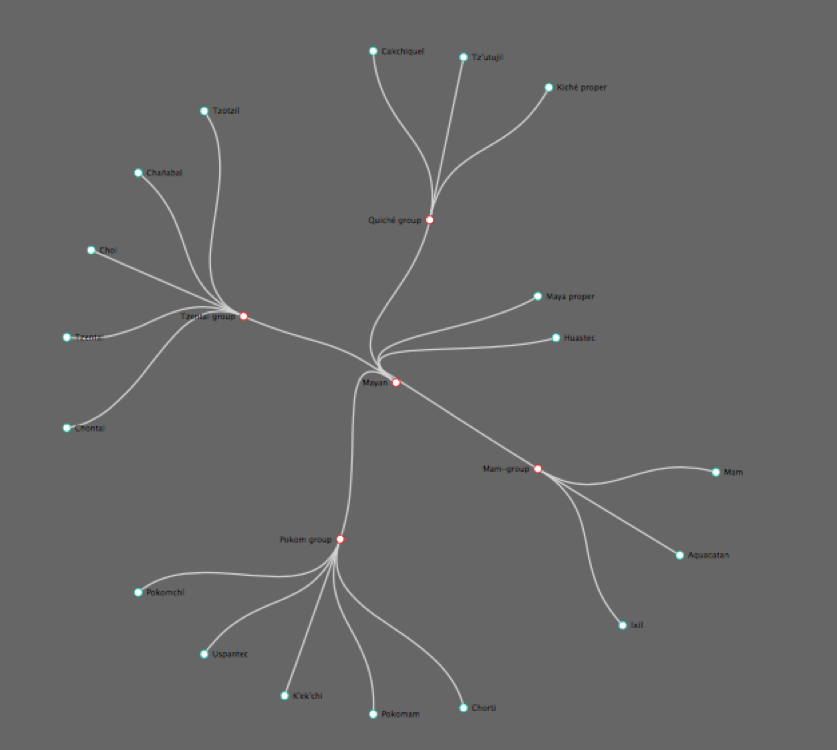
\includegraphics[scale=0.8]{figures/gatschet1895.png}
    \caption{Gatschet (1895), according to \citet{GatschetCampbell1973}. This is the radial view with descendants expanded. Available at: \url{http://new.multitree.org/trees/id/21186}}
    \label{fig:kaplan:gatschet}
\end{figure}

Why bother layering the biosystematic metaphor on top of the familial (see \citealt[49]{Wells1987} on ``mixed metaphors'', 53--54 on biological imports)? When it comes to MultiTree, this choice not only fosters comparability across the database, it also reflects architects' stated commitments to aesthetics, access, and ``fun''. In other words, the visual is second nature to those already familiar with the techniques of comparison and sub-grouping, and it recruits potential newcomers to those particular methodological approaches.

This brief example is meant to suggest that tree thinking did not have a necessary or inevitable trajectory in comparative-historical linguistics. Trees were not the only means available for the organization of information on ancestor-descendant relations.\footnote{The case in biology on this point is somewhat different. In the case of Lamarck's diagrams, for example, the shift from tables (e.g. 1778) to trees (e.g. 1809) coincided with a definite conceptual shift (re. species mutability). The recognition of variation and change over time did not correspond with the visual in linguistics \citep[ch. 3]{Archibald2014}.} Rather, they have served additional rhetorical purposes, taken up in the next section.

\section{Canonical visual metaphors}
\label{sec:kaplan:visualmetaphors}

1853 was a pivotal year with regard to the visualization of language relationship — two of the earliest known language family trees were published that year.\footnote{In fact, the ``Arbre Généologique'' by Felix Galet (ca. 1807) is often cited as the first tree of language relationship \citep[242]{Hellstrom2012}. This chronology roughly aligns with the biological context, where the first known tree diagram of relationship was published by Augustin Augier in 1801.} The first, posthumously attributed to the Czech poet and translator Frantiek Ladislav Čelakovský (1799—1852), depicted the historical differentiation of the Slavic language family (\citealt[3]{Czelakovsky1853}; \citealt{Priestly1975}). But Čelakovský's contribution has been overshadowed by the trees of August Schleicher (1821—1868). His first such visualization depicted the Indo-Germanic family with thick branches and weighty arboreal realism (see \citealt{Maher1966}; \citealt{Hoenigswald1975}; \citealt{Koerner1987}). Significantly, Geisler and List suggest that this diagram was a formalization, after the fact, of Schleicher's first published reflections on the comparative history of languages some five years earlier \citep{Schleicher1848}. Identifying relationship with descent, and pinning that conception on the tree, they assert, Schleicher's ``new theory of vertical language relations [was] directly reflected in the tree model'' that has since become so familiar \citep[114]{GeislerList2013}.

What more did Schleicher invest in his ``schema'' than a procedure for classification by two-way splits? Historians have emphasized notions of parsimony, regularity \citep[117, 114--115]{GeislerList2013}, organicism \citep[56]{Wells1987}, and programmatic ambition \citep[755]{Koerner1975}. More concretely, Schleicher told readers directly that branch length served as an indicator of ``duration'' and that the distance between branches was meant to indicate ``degrees of relationship'', left otherwise undefined \citep[8]{Schleicher1853}. Going further, Schleicher emphasized the importance of his trees for training newcomers to the field, and their projected departure from older philological traditions:

\begin{quotation}
In the present work an attempt is made to set forth the inferred Indo-European original language side by side with all extant derived languages. Besides the advantages offered by such a plan, \emph{in setting immediately before the eyes of the student the final results of the investigation in a more concrete form, and thereby rendering easier his insight into the nature of a particular Indo-European language}, there is, I think, another advantage of no less importance, namely that it shows the baselessness of the assumption that the non-Indian Indo-European languages were derived from Old-Indian (Sanskrit), an assumption which has not yet entirely disappeared. \citep[94]{Schleicher196718612}
\end{quotation}

My emphasis on the first ``advantage'' described in this passage, the pedagogical advantage, presents the tree diagram as tool for summing up and disseminating research findings to those just entering the field — for Schleicher it was decidedly \emph{not} a means to new linguistic knowledge. References to the ``eyes'' and ``insight'' of the student recall Daston's (\citeyear{Daston2008}) depiction of the ``all-at-once-ness'' of disciplined perception, seen here to be very much in the making through the association between pedagogy and disciplinary differentiation. That said, phylogeny does not appear to be a primary goal, in and of itself. Rather, it is celebrated as a means to better understand a ``particular'' language under investigation. Schleicher's philosophy of science did not necessarily demand knowledge of a general sort \citep{Nyhart2012}. His visual epistemology appears to have involved a kind of inward tendency, from sight to insight, both in the cultivation of the student and the discipline.

By the early 1870s, the outlines of the Indo-European family had been drawn, giving comparativists considerable cause for celebration. Nevertheless, exceptions persisted. As a young professor of German and Slavic at the University of Bonn, Johannes Schmidt (1843—1901), a student of Schleicher's, tackled these difficulties head-on. In a 31-page monograph on \emph{The Relationships of the Indo-Germanic Languages} [\emph{Die Verwandtschaftsverhältnisse der indo\-ger\-manischen Spra\-chen}], he demonstrated that unique resemblances can be identified between any two Indo-European branches, and that these tend to increase with geographic proximity. In light of this observation, he argued that linguistic changes spread laterally like waves on a pool of geographically distributed speech, rather than vertically, through a process of strict cleavage and differentiation. With each change distributed individually, he projected an image of successive waves moving out and interacting from a variety of centers -- a network of linguistic features differentiated through space.

Though Schmidt did not give readers a diagram of his \emph{Wellentheorie} in 1872, he did picture it in words.\footnote{The critique of Schleicher's tree thinking through alternative visual metaphors came even earlier in Hugo Schuchardt's 1870 lecture ``On the Classification of the Romance Dialects'', where he speaks of killing the tree by binding together numerous branches and twigs with ``horizontal lines'' \citep[11]{Schuchardt19001870}.} With the following passage, Schmidt invited readers to join him in an image metaphor:

\begin{quotation}
If we want now to represent the relationships of the Indo-Germanic languages in a picture that illustrates the origin of their diversity, then we must completely abandon the idea of a family tree. I would like to \emph{put a picture of a wave in its place}, which diffuses concentrically with the distance from the mid-point in ever weaker rings. It does not matter that our language area makes no circle, rather a circle-sector at best, with the most primitive language at	one end, not the centre […] There were not initially any boundaries between languages within this domain, two arbitrarily distant dialects, A and X, were connected to each other by continuous varieties, B, C, D etc. […] \citep[27--28]{Schmidt1872}\footnote{``Wollen wir nun die verwantschaftsverhältnisse der indogermanischen sprachen in einem bilde darstellen, welches die entstehung irer verschidenheiten veranschaulicht, so müssen wir die idee des stammbaumes gänzlich aufgeben. Ich möchte an seine stele das bild der welle setzen, welche sich in concentrischen mit der entfernung vom mittelpunkte immer schwächer werdenden ringen ausbreitet. Dass unser sprach-gebiet keinen kreis bildet, sondern höchstens einen kreissector, dass die ursprünglichste sprache nicht im mittelpunkte, sondern an dem einen ende des gebietes ligt, tut nichts zur sache […] Sprachgrenzen innerhalb dises gebietes gab es ursprünglich nicht, zwei von einander beliebig weit entfernte dialekte des selben A und X waren durch continuierliche varietäten B, C, D, u.s.w. mit einander vermittelt.''} 
\end{quotation}

With references to ``pictures'', geometry, and dialect labels, this passage reads as though it were captioning a printed diagram, though Schmidt did not provide one at first to accompany the text. Indeed, he went on to challenge the visual altogether -- asserting the priority of linguistic data over any such formalization. As far as he was concerned, ``[p]ictures have only marginal value in science, and if the one chosen here is displeasing to someone, he can replace it at will with something better without changing the results of the foregoing analysis''.

Perhaps this attitude partly explains why his first attempt to provide a visual aid lagged some three years behind his introduction of the image metaphor. Perhaps this reluctance derived from problems inherent to the visualization of horizontal relationship. Geisler and List suggest as much through their side-by-side presentation of several ``fruitless'' attempts to draw an alternative to Schleicher's trees -- from overlapping circles \citep{Hirt1905}, to the spokes of a wheel \citep{Meillet1908}, to early networks \citep{bonfante1931}, and alternating boundaries \citep{Bloomfield1933}. I turn now to the challenging case of another visual metaphor that attempted to capture vertical and horizontal relationship simultaneously.

\begin{figure}
    \centering
    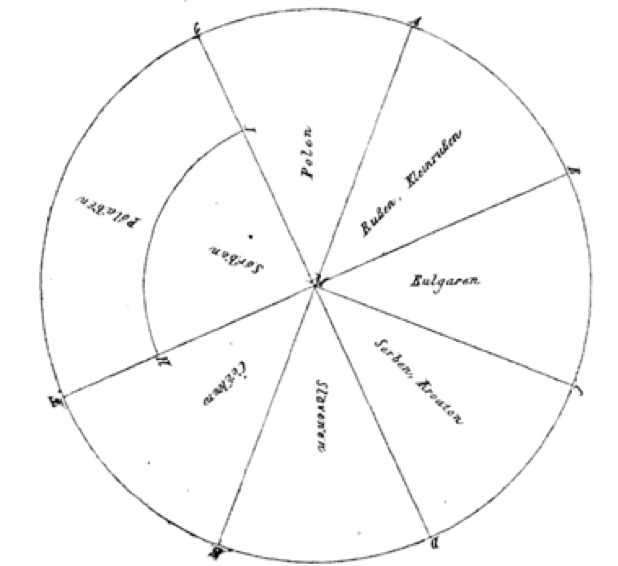
\includegraphics[scale=1]{figures/schmidt1875.png}
    \caption{\citet[199]{Schmidt1875}. The text goes on to tell readers that the radia between lettered points should be read as isogloss lines, carving out dialects like pieces of a pie.}
    \label{fig:kaplan:schmidt}
\end{figure}

J. Heinrich Hübschmann (1848--1908) heeded Schmidt's call to data-driven analysis in his comparative work on Armenian. Like Schmidt, Hübschmann studied with Schleicher at the University of Jena, though he later completed his degree under the Iranian philologist Martin Haug (1827—1876) at the University of Munich. Having defended a dissertation on Avestan and Old Persian philology in 1872, he turned in the next three years to an investigation of the relationship between Iranian and Armenian in pursuit of his Habilitation at the University of Leipzig. Initially, Hübschmann was only interested in Armenian insofar as it contributed to an understanding of the internal phylogeny of the Iranian family of languages. In line with the general consensus of the day, Hübschmann had, up to this point, taken a high degree of shared vocabulary as evidence of the fact that Armenian was part of Iranian \citep{Schmitt1976}.

His postdoctoral studies culminated in the \citeyear{Huebschmann1875} paper ``On the Position of Armenian in the Circle of the Indo-Germanic Languages'' [\emph{Ueber die Stellung des Armenischen im Kreise der indogermanischen Sprachen}]. Here Hübschmann sorted out non-native parts of the lexicon and analysed the remaining ``native'' words, which allowed him to identify strata in the historical development of the language. His findings compelled his colleagues to recognize Armenian as an independent branch of the Indo-European family — not a sub-group of Iranian after all.

In the \citeyear{Huebschmann1875} essay, Hübschmann demonstrated an extensive political history of contact and exchange between native Armenian-speaking and Iranian-speaking groups, suggesting that the similarities traditionally invoked in support of the ``prevailing'' view of common descent were in fact derived from the sector of borrowed, not inherited, vocabulary. Working back and forth between etymological and phonological evidence, Hübschmann next established provisional sound laws unique to Armenian, which undermined long-standing confidence in what were thought to be cognates between the languages in question. From the lexicon, Hübschmann then moved to grammatical considerations -- the inflectional morphology of Iranian and Armenian, which exhibited many surface similarities. He attributed these to processes of analogical change -- a psychological process of association tending to regularize words with similar meanings or inflectional paradigms, a mechanism of convergence.

Adding further phonological evidence to the balance against family relationship in this case, Hübschmann came to a fairly radical position, one that prioritized horizontal over vertical relationship:

\begin{quotation}
Through the last part of our investigation, such a tight bond has without question been constructed between Armenian and European that it would be easier to tear Armenian from Aryan than from European. Among the European languages it stands closest to Balto-Slavic […] In this situation, friends of the family tree […] will certainly be inclined to separate Armenian completely from Aryan and make it a purely European language. Against this view I might first refer to the fact that Armenian does not take part completely in the split of \emph{a} and \emph{r} […] 

If further research makes this conclusion definitive, then the impossibility of setting up a family tree of the Indo-European languages would be strikingly demonstrated. For Armenian would be the connecting ring of both parts in the chain of the Aryan-Balto-Slavic languages, not a branch between two branches. And then too the family tree, which Johannes Schmidt's vigorous might has overturned, would remain lying forever […] 

But if Armenian is to be the connecting member between Iranian and Balto-Slavic, between Aryan and European, then in my opinion it must have played the role of an intermediary at a time when they were still very similar to one another, when the historical period had not yet drawn the present sharp boundary between them, but when they were still related to one another as dialects. \citep[183]{Huebschmann1875}
\end{quotation}

Like all the examples encountered thus far, Hübschmann appealed first to a visual metaphor in this passage rather than a visual aid. Further, his discussion highlights inherent difficulties in drawing vertical and horizontal relationship together. To see Armenian as a link in the chain between Aryan and European, it was necessary to focus in on ``\emph{a time} when they were still very similar''. If trees lacked, fundamentally, a feeling for spatially distributed variation, waves were completely without a sense of timing.

Though this painstaking work secured Hübschmann's reputation as the ``father'' of modern Armenian linguistics -- a doubly genealogical claim -- previous accounts have not had much to say about the degree to which his positivism paradoxically threatened to topple his faith in the comparative method. In a paper ``On the pronunciation and transcription of Old Armenian'', published the following year, Hübschmann pushed Schmidt's visual still further:

\begin{quotation}
[…] it seems that languages can have similar sound systems without being related to one another, that the sound system of a language by others, i.e. local influences can be assumed, leading one to infer the congruencies between the sound systems of two languages less from their origin as from their local gathering. This statement seems to me for the determination of the genealogy of languages to be important and in linguistics to reward further success than heretofore was the case [… I]f Iranian languages on the border of India show Indic sound similarities, must one therefore believe that they stand nearer to the Indic than the other Iranian languages? \citep[66]{Huebschmann1876}\footnote{``Aus alledem ergiebt sich, dass Sprachen das gleiche Lautsystem haben können, ohne miteinander verwandt zu sein, dass das Lautsystem einer Sprache von äusseren, d.~h. localen Einflüssen bedingt sein kann, und man aus der Gleichheit des Lautsystems zweier Sprachen weniger auf ihre Verwandtschaft als auf ihr locales Beisammensein zu schliessen hat. Dieser Satz scheint mir für die Beurtheilung der Verwandtschaftsverhältnisse der Sprachen wichtig zu sein und in der Linguistik mehr Beachtung zu verdienen als es bisher der Fall war. Also, um unsern Satz auf einen Fall anzuwenden: wenn iranische Sprachen an der Grenze Indiens indische Lauteigenthümlichkeiten (durch den Gebrauch von Lingualen und Aspiraten) zeigen, hat man darum zu glauben, dass sie dem Indischen näher als die andern iranischen Sprachen stehen?''}
\end{quotation}

Evidently, the dictates of historical fidelity required taking vertical \emph{and} horizontal relationship into consideration. But this proved remarkably difficult to capture visually. Hübschmann's best practice was to toggle back and forth between the two.

\section{Metaphors and visual aids in twentieth-century textbooks}
\label{sec:kaplan:textbooks}

The canonical topoi just considered enjoyed a hearty afterlife in the \emph{Disziplin\-geschichte} of the late nineteenth century, and its review in textbooks thereafter. This section looks at the deployment of visual aids in that genre, building on previous studies of print and pedagogy in the history of chemistry, physics, and biology (\citealt{bertomeusanchez2002}; \citealt{Kuhn1962}; \citealt{Hopwood2015}). This literature has shown how scientific textbooks specialized from the late eighteenth century on, emphasizing their ``use in formal teaching and their pedagogical and scientific authority''; their significance for disciplinary self-fashioning; and their ``major role'' in the making of \emph{interactional expertise}, that is ``the worldviews of citizens, what they know, what they do, what they are'' (\citealt[475, 479]{Simon2016}; \citealt[406--408]{Johns1998}).\footnote{Josep \citet{Simon2016} contends that ``textbook'' had come to mean a book conceived for instructional purposes within formal education by the middle of the nineteenth century, picking up on the earlier convention of designating canonical works, excerpted with spaces for students' interlineal notes, as \emph{texts}. Thus, he implies a direct connection between the history of note-taking practices and the development of formal, printed textbooks. This contextualizes John Joseph's compelling \citeyear{Joseph2017} discussion of the ambiguous relationship between pictures and words in Saussure's \emph{Cours de linguistique généale} within a broader history of science and education.}

Leonard Bloomfield's \emph{Language} met all of these criteria: it served as a provocative introduction to descriptive linguistics in \citeyear{Bloomfield1933}, asserting a new program while disciplining perception \citep[v-vi]{BloomfieldHoijer1965}. Comparative-historical material, notably, bookends the text: it appears first as a kind of ``preface history'', recounting progress toward the modern ``scientific'' study of language, and in the second half of the book, aligning with Bloomfield's priorities and programmatic vision. Far from a straightforward reproduction of earlier works, the presentation of historical research in the later part was designed for American students -- those just beginning linguistics ``who often d[o] not have the background in Indo-European languages'' necessary to ``understand texts that present methodology very largely in terms of concrete problems drawn from the older Indo-European languages'' \citep[vi]{BloomfieldHoijer1965}. Put differently, the update shifted from exemplars to models, in line with what could reasonably be assumed of a new generation of students.

What, then, was textually self-evident, and what did Bloomfield think needed elaboration through the use of visual aids? By far the most common diagram in \emph{Language} is the table, followed by maps (eight), and only then abstract visualizations of the sort laid out in the previous section. Interestingly, Bloomfield identifies visual metaphors and visual aids in teasing out the implications of the former. Students read:

\begin{quotation}
The comparative method assumes that each branch or language bears independent witness to the forms of the parent language, and that identities or correspondences among the related languages reveal features of the parent speech. This is the same thing as assuming, firstly, that the parent community was completely uniform as to language, and secondly, that this parent community split suddenly and sharply into two or more daughter communities, which lost all contact with each other. Often enough, the comparative method assumes successive splittings of this sort in the history of a language […] The comparative method thus shows us the ancestry of languages in the form of a family tree, with successive branchings […]  \citep[311]{Bloomfield1933}
\end{quotation}

This passage rehearses standard criticisms of the tree model — namely, ancestral uniformity and clean two-way splits — showing it to have heuristic power despite being unrealistic. Thus, it signals an advance over nineteenth-century understanding. ``The earlier students of Indo-European did not realize that the family-tree diagram was merely a statement of their method; they accepted the uniform parent languages and their sudden and clear-cut splitting as historical realities'' \citep[311]{Bloomfield1933}. In this way, Bloomfield subordinated Schleicher's visual aid to a method of inference. Translating this into Lakoff's terminology, an ``image metaphor'' moved toward the ``conceptual'' register.

\begin{figure}
    \centering
    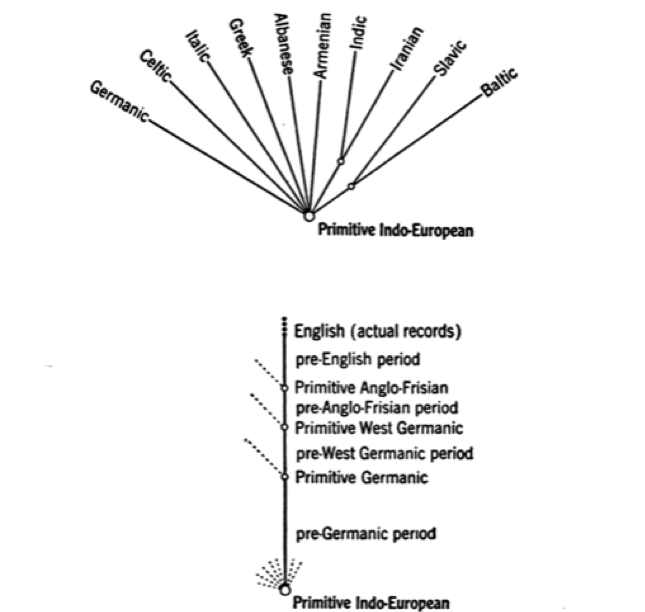
\includegraphics[scale=1]{figures/bloomfiield1933.png}
    \caption{\citet[312]{Bloomfield1933}}
    \label{fig:kaplan:bloomfield}
\end{figure}

This shift was reflected in the highly idealized visual that accompanied the text, shown in Figure~\ref{fig:kaplan:bloomfield}. The lengths and distances between branches are not particularly measured, and the labels refer to groupings and periods rather than specific language entities. Bloomfield was an anti-realist tree thinker, to be sure: the diagrams above depict relations but not relatives.

In the text, Bloomfield persistently refers tree thinking to ``older scholars'', setting off his positive variationist approach. To complement a series of examples highlighting exceptions to the assumption of clean two-way splits, he adapted a visual aid from the Germanist and linguistic paleontologist Otto Schrader (1855--1919), shown in Figure~\ref{fig:kaplan:schrader}.

\begin{figure}
    \centering
    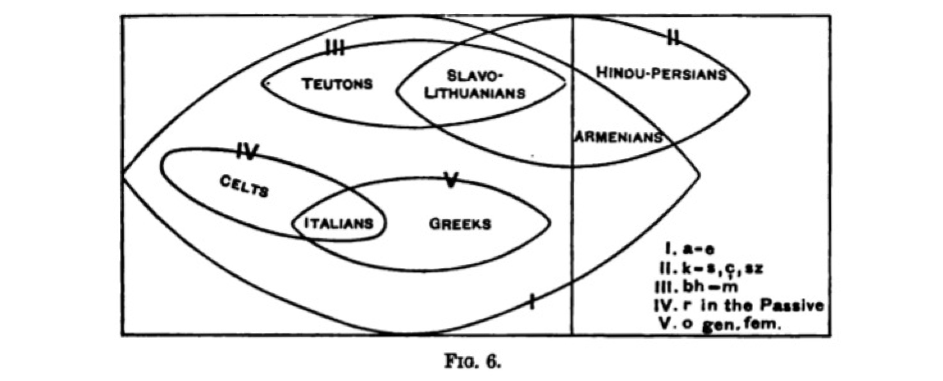
\includegraphics[scale=0.8]{figures/schrader1890.png}
    \caption{\citet[65]{Schrader1890}}
    \label{fig:kaplan:schrader}
\end{figure}

\begin{figure}
    \centering
    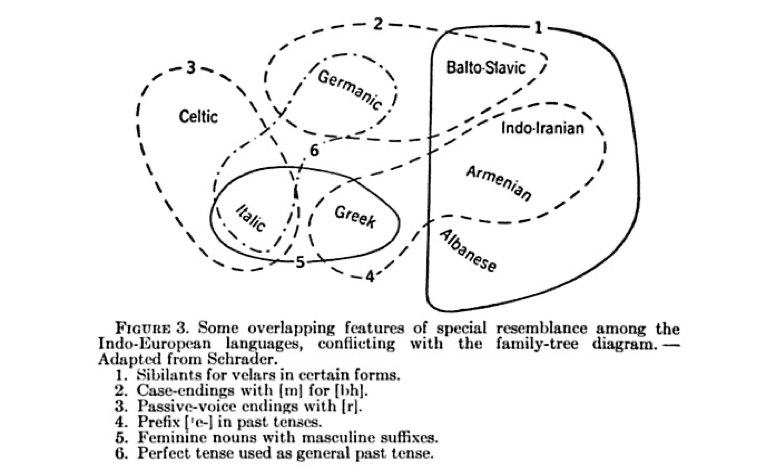
\includegraphics[scale=1]{figures/bloomfield1933-316.png}
    \caption{\citet[316]{Bloomfield1933}}
    \label{fig:kaplan:bloomfield316}
\end{figure}

The citation to Schrader may at first seem surprising, given that the authors differ in their selection of ``special resemblances'', hence, group assignments \citep[317]{Bloomfield1933}. However, both authors allow that the groups could be drawn differently depending on the forms taken into consideration. Bloomfield explained his image in Figure~\ref{fig:kaplan:bloomfield316} -- containing elements of uniformity and variation -- in terms of Schmidt's ``\emph{wave-hypothesis}'', which he endorsed. ``Indeed'', he wrote favourably, it is ``the picture presented by the local dialects in the areas we can observe'' \citep[317]{Bloomfield1933}. Charles Hockett (1916--2000), writing in a more richly visual idiom some twenty-five years later, would refer a reprint of the same image to overlaid notions of vertical and horizontal relationship \citep[cf.][]{Huebschmann1875}.

Bloomfield's influence can be seen throughout the pages of Hockett's textbook, \emph{A Course in Modern Linguistics} (\citeyear{Hockett19591958}). Hockett introduced his subject in rigorous terms: ``Linguistic research can accomplish nothing unless it is strictly inductive'' \citep[7]{Hockett19591958}. Such primacy of ``actual usage, as determined by observation'' was born out in the sequence of chapters, which proceed from the smallest units of synchronic observation -- defined through examples and presented with rules for exacting description -- to the more complex, with chapters on language diachrony and other un-observables saved for the end. Indeed, he did not even mention the distinction between synchronic and diachronic linguistics in the book until Chapter 36.

There are clues to Hockett's visual epistemology throughout the text, with bearing on the way he called upon diagrams of language relationship. First, the text shows a remarkable tolerance for the kind of idealization any visualization of language relationship would require. Elaborating on the ``design of a language'' through its five subsystems, he allowed, for instance, that no description ``can claim more than a kind of by-and-large accuracy'' \citep[139]{Hockett19591958}. He similarly flagged the underdetermined and heuristic nature of grammatical description in connection with immediate constituents a few pages later. The following passage is perhaps unexpected behaviourist fare:

\begin{quotation}
[…] grammatical analysis is still, to a surprising extent, an art: the best and clearest descriptions of languages are achieved not by investigators who follow some rigid set of rules, but by those who through some accident of life-history have developed a flair for it […] Consequently, the reader will find in these sections many an example which the writer has handled in one way, but which might also be handled in some other way […] Indeed, the reader should be alert for possible instances where conciseness of statement has unintentionally concealed uncertainty.  \citep[147]{Hockett19591958}
\end{quotation}

Reflections like these contextualize his use of visual metaphors (e.g., the persistent reference to phonemic ``shape'') and visual aids in the text \citep[130--132]{Hockett19591958}. With respect to the latter, Hockett's use of two-dimensional abstract representations involved explicit pedagogical aims. For example, in the notes to his chapter on ``Canonical Forms and Economy'', Hockett taught students \emph{how to see} the three diagrams in Figure~\ref{fig:kaplan:hockett1959291} which were most often used to represent complex morphological systems — the ``maze'', ``freightyard'', and ``rollercoaster'' (\citealt[290-292]{Hockett19591958}; \citealt{Harris1951}; \citealt{Hoenigswald1950}).

\begin{figure}
    \centering
    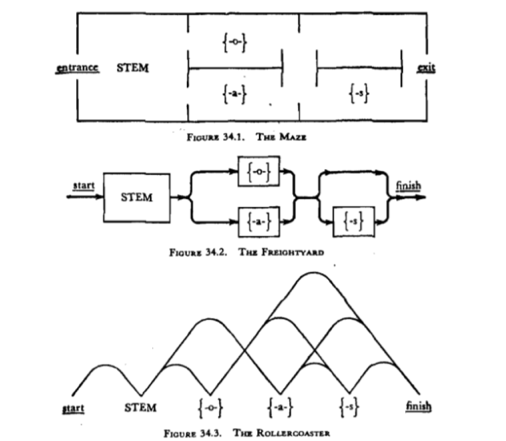
\includegraphics[scale=1]{figures/hockett1958-291.png}
    \caption{\citet[291]{Hockett19591958}}
    \label{fig:kaplan:hockett1959291}
\end{figure}

Hockett told readers that the example provided was derived from the inflection of gendered Spanish adjectives, a pattern ``too simple to need diagrammatic display'', thus a ``good one with which to demonstrate the diagramming techniques''. The words accompanying these images train students in the techniques of visual analysis -- navigating the maze, for example, one proceeds ``from left to right, never crossing any lines''; once in the freightyard, there is ``no turning back''; and while riding the rollercoaster, ``one can turn down wherever there is a curved top, but not an angle''. Thus, Hockett formalized morphological rules, rendered them exhaustive, and made them intelligible for beginners. The penultimate paragraph on the matter provides lessons in \emph{critical} visual analysis. Here Hockett pointed out that vertical alignment in the first two diagrams can be ``read'' as indicating ``a single positional class'', whereas the ``rollercoaster has the advantage of listing all the inflectional affixes along the bottom for ease of checking against inadvertent duplications''. The discussion concludes with an exercise that recruits students to the practice of diagrammatic visualization, suggesting that this was not merely a means of summing up, but rather an active part of research practice.

How was this visual epistemology brought to bear on questions of language relationship? Hockett defined relationship in terms of common origin: divergence being the key factor, not time. Accordingly, he made a sharp distinction between linguistic and biological phylogeny -- ``languages do not `reproduce' either sexually or asexually'', instead, they ``simply \emph{continue}'' \citep[369]{Hockett19591958}. For this reason, familial metaphors to do with parenthood and ancestry appeared ``shaky'' in his estimation. ``At a given point in time,'' he concluded,

\begin{quotation}
a set of related languages is merely what would be a set of dialects of a single language except that the links between the dialects have become very tenuous or have been broken […] The mere fact of relationship thus becomes of secondary importance. More important is the \emph{degree} of relationship. \citep[369]{Hockett19591958}
\end{quotation}

The first tree diagrams to appear in the text serve methodological rather than representational ends. Grouping together Proto-Germanic and its descendants without concern for sub-grouping, two sets of arrows in Figur~\ref{fig:kaplan:hockett1959514} instead illustrate the logic of traditional and inverted reconstruction.

\begin{figure}
    \centering
    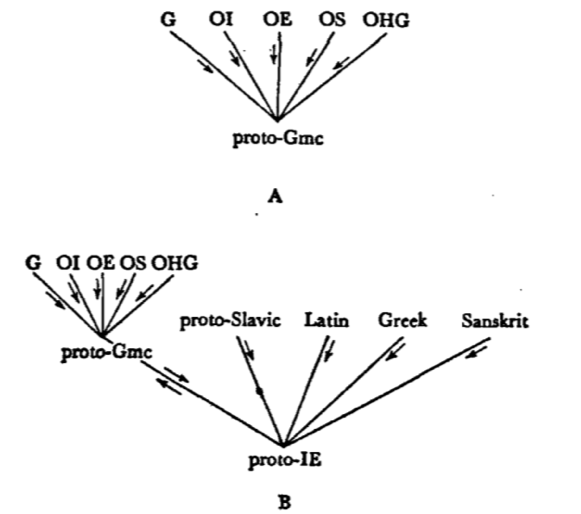
\includegraphics[scale=1]{figures/hockett1958-514.png}
    \caption{\citet[514]{Hockett19591958}}
    \label{fig:kaplan:hockett1959514}
\end{figure}

A more realistic tree diagram, reproduced in Figure~\ref{fig:kaplan:hockett1959519}, appears a few pages later, qualified, with tips on interpretation.

\begin{figure}
    \centering
    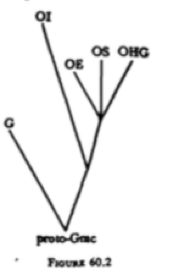
\includegraphics[scale=1]{figures/hockett1958-519.png}
    \caption{\citet[519]{Hockett19591958}}
    \label{fig:kaplan:hockett1959519}
\end{figure}

Of this canonical image, Hockett wrote:

\begin{quotation}
The vertical dimension represents time, increasing as one goes from bottom to top. G has been placed earlier than the other four languages because our records of it date from an earlier century. Read literally, the diagram would suggest that, after Proto-Germanic, first the speakers of what was to become G split off from the rest […], that somewhat later the speakers of what was to become OI moved away from the rest, and that, finally, the remaining group split three ways — the splits, in each case, being more or less sudden. Now such literal interpretation is not contrary to what sometimes happens in history. But it is dangerous to assume that this is always what happened, because there are other ways in which divergence can come about.  \citep[519--521]{Hockett19591958}
\end{quotation}

This passage begins with extremely rudimentary visual directives, a reminder of the pedagogical aim of the work. It also says something — through reference to ``our records'' -- about the research labour that goes into ``cooking'' the data summarized by the family tree. From there, readers are directed through a ``literal'' reading of the tree. The important point here is that insights on historical \emph{process} are being extracted from a given \emph{pattern} of historical relationship. While a bracketed table might capture a similar classification of language relationship, it would be harder to read in such a richly narrative way. This is because it would lack the ``entailments'' of the underlying image and conceptual metaphors we have been tracing. Ultimately, Hockett concluded, the tree was a possible, but unrealistic way of representing relationship. ``It is imperative for us to remember that our reconstruction wears a disguise of greater preciseness than can validly be ascribed to it, but to throw it out for this reason would be folly'' \citep[523]{Hockett19591958}. He proposed the alternative illustrated in Figure~\ref{fig:kaplan:hockett1959520} instead.

\begin{figure}
    \centering
    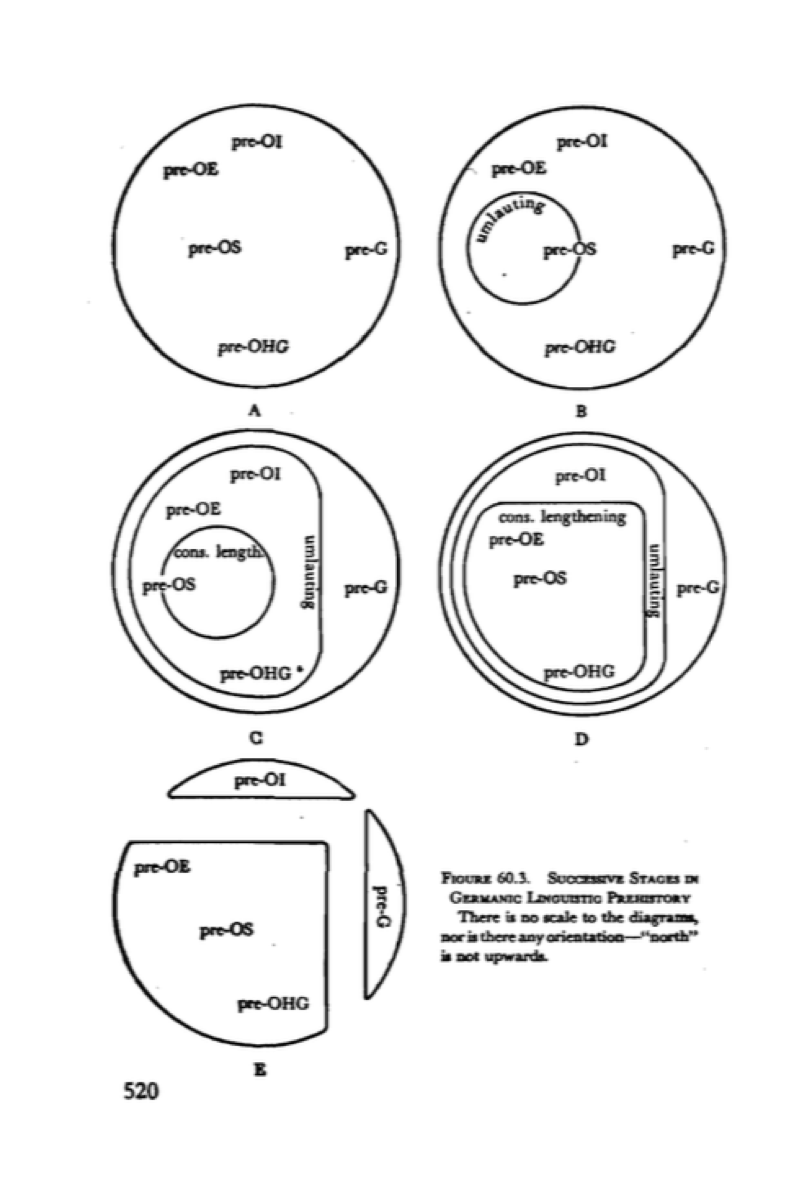
\includegraphics[scale=0.8]{figures/hockett1958-520.png}
    \caption{\citet[520]{Hockett19591958}}
    \label{fig:kaplan:hockett1959520}
\end{figure}

The diagram in Figure~\ref{fig:kaplan:hockett1959520}, in effect, zooms in on the base of the previous tree, looking at it through a series of cross-sectional slices like a flip-book. A succession of slices was Hockett's best effort to visualize relationship simultaneously in space and time. It culminated in the recapitulation of Bloomfield's diagram of dialect geography, formulated here in the context of a methodological argument rather than a list of discrepant data. This reflects another step away from exemplary towards formal instruction.

In his overview of scientific textbooks, Josep Simon calls for a transdisciplinary exploration of the genre, beyond a traditional emphasis on disciplines and discipline-formation in connection with this site of ``normal science'' \citep[475]{Simon2016}. In partial fulfilment of that call, the final example in this section pivots from general introductions to a textbook devoted specifically to the sub-discipline in question, Theodora Bynon's \emph{Historical Linguistics} (\citeyear{Bynon1977}). Significantly, Bynon introduces the twentieth-century organization of linguistic knowledge with an extended image metaphor:

\begin{quotation}
The representation of the evolution of a language as consisting in a succession of discrete states is no more a true reflection of the situation than is the representation of a circle by a number of straight lines connecting successive points around its circumference. For, however large a number of such points are taken the resulting figure will never be a genuine circle and, in the same way, however many language sates are considered over a given period their succession will never provide a true picture of the unbroken \emph{continuity} of a language in time. It is thus due to the limitations of our methodology that we are faced with the rather absurd situation that language evolution, although observable retrospectively in its \emph{results}, appears to totally elude observation as a \emph{process} while it is actually taking place. \citep[2]{Bynon1977}
\end{quotation}

So much for any attempt to comprehend, let alone visualize or represent, historical products and processes realistically. Accepting this fate, Bynon accordingly opts for a ``two-fold strategy''. First, she presents models of linguistic development from the neogrammarians to the transformational-generative school. ``We must study [the] results [of language change] as abstracted from the grammatical descriptions of successive language states and […] of related languages'' \citep[6]{Bynon1977}. Second, she turns to the ``question of the connection between language change and social and geographical space'' \citep[6]{Bynon1977}. Rather than worry about the historical fidelity of either approach to the study of relationship and differentiation, this text holds them apart schematically.

\begin{figure}
    \centering
    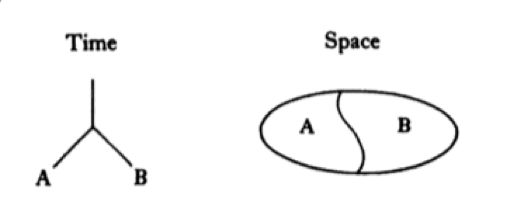
\includegraphics[scale=1]{figures/bynon1977.png}
    \caption{\citet[173]{Bynon1977}}
    \label{fig:kaplan:bynon1977}
\end{figure}

According to this overall scheme, questions of the linear development of language through time -- and, with them, trees -- are isolated from those pertaining to internal variation and contact. Trees appear in her narrative as a bridge from the consideration of change within individual languages to changes between them. For Bynon, trees are not primary, they do the work of summing up the ``rules'' of differentiation -- a sign of her times. That said, she emphasizes their visual interpretation more than either Bloomfield or Hockett. Describing a downward branching tree linking English, German, the Greek dialects, Persian and Sanskrit back to Proto Indo-European through a series of innovations, students read:

\begin{quotation}
In the tree diagram the horizontal dimension […] represents ``space'' in a much idealized form -- not in an absolute geographical sense but rather in terms of contact or absence of contact between speech communities -- whereas the vertical dimension represents time. The branches of the tree then represent channels of transmission, that is the paths along which innovations have been transmitted, and whenever a branch divides into two or more this implies the splitting up of a speech community indicated by the fact that subsequent innovations are no longer shared. \citep[66]{Bynon1977}
\end{quotation}

Clearly, Bynon embraced anti-realistic tree thinking, though here she invests more words in training students to see this model than her structuralist predecessors. Notably, she resists the urge to conclude her discussion with an all-inclusive diagram of the Indo-European family, opting for a two-page chart instead, shown in Figure~\ref{fig:kaplan:bynon197768}.

\begin{figure}
    \centering
    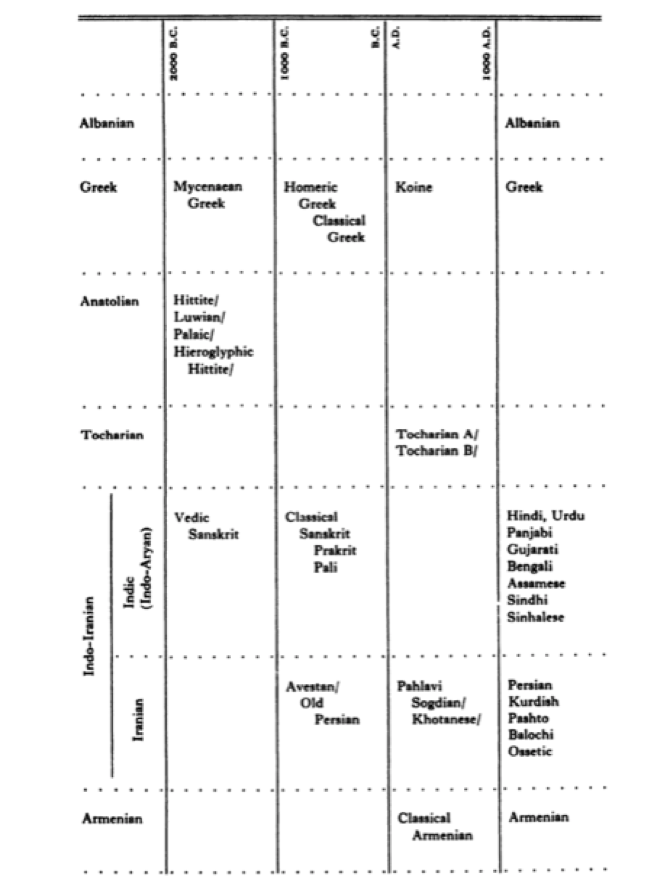
\includegraphics[scale=1]{figures/bynon1977-68.png}
    \caption{\citet[68]{Bynon1977}. This is half of the chart, which stretches over two pages.}
    \label{fig:kaplan:bynon197768}
\end{figure}

This diagram, she concludes, has the advantage of not overstating putative relationships, designed, as it was, to bring ``together loosely according to branches and periods the main languages of the Indo-European family for which actual material survives.'' As for the tree model, Bynon states, it should be reserved for ``the display of rules relating successive systems'' \citep[70]{Bynon1977}. At roughly the same time as phylogenetic modelling was taking off in biology, Bynon was relinquishing the analogy between languages and biosystematics entirely.

\section{From anti-realism to realism in the digital era}
\label{sec:kaplan:realism}

At a 1973 conference on the topic of ``Lexicostatistics in Genetic Linguistics'', convened in Montreal, Paul Black presented a paper on the adaption of Multidimensional Scaling (\textsc{mds}) to historical linguistics, which built on a prior collaboration with Isidore Dyen and Joseph Kruskal of Bell Labs. His work was an early attempt to model hybrid transfer computationally using data collected by others. Black endorsed the controversial use of statistics in comparative-historical linguistics, stating by way of introduction that metrical analysis of linguistic distance ``permits a multidimensional recognition of relations'' \citep[43--92]{Black1973}. Thus, Black adapted canonical metaphors of language relationship -- forged on the basis of Indo-European data in a two-dimensional environment -- to a new geographic and conceptual space.

Carried over from the world of marketing, psychology, and political science, Black described \textsc{mds} as a way to see continuous variation (``cline structure'') within a hierarchy of discrete classes (the evolutionary tree).  The objective was hybrid in nature:

\begin{quotation}
While a ``family tree'' diagram or some other representation of a hierarchical subgrouping is an obviously appropriate way of describing the temporal hierarchy of linguistic splits through which a group of languages may have evolved from a common ancestral protolanguage, multidimensional scaling can be used to investigate and describe the spatial variation which originates in the wave-like spread of linguistic innovations within a single language, and which may also persist within the evolutionary tree to an extent sufficient to hamper the correct inference of this tree.  \citep[43]{Black1973}
\end{quotation}

According to Black's discussion, the method was new in that it began by \emph{testing} -- rather than assuming or imposing -- the fit between tree classifications, wave models, and the actual language data (in this case, pertaining to Bikol, Lower Niger dialects, Konsoid, and Salish) they were meant to represent. From there, distances between each of the entities under consideration (dialects or languages) were scaled so as to approximate ``actual physical distances''. Looking at Bikol dialects, for example, one might figure percentages of lexicostatistical retention, subtract each from one hundred percent, and map each percentage point of difference as a distance of one tenth of an inch. A common retention of 79\%, as in the case of Sorsogon and Masbate, for instance, might yield a one-dimensional distance of 2.1 inches according to this method. Black continued,

\begin{quotation}
Oas might then be added to the picture by placing it 3.1 inches (corresponding to 69\%) from Sorsogon and 4.2 inches (corresponding to 58\%) from Masbate; these relationships would then be well represented in two-dimensional space as a triangle. \citep[52]{Black1973}
\end{quotation}

This was reasonably straightforward. But, as Black pointed out, the procedure becomes increasingly unwieldy as more dimensions are added to the mix, such that the representation ``might prove to be difficult to visualize and interpret'' should dimensionality not be ``restricted to some very small number'' \citep[53]{Black1973}. With these words, Black was confronting the difficulty of reconciling language data with formalized relationships, fidelity with the ``all-at-onceness'' of disciplined perception. Even if \textsc{mds} was escaping the constraints of the printed page as a research tool, Black was still bound to two dimensions when it came to the communication of research findings. In order to flatten a full set of distance measures into a two-dimensional representation with some degree of intelligibility, it was necessary to adjust the original percentages in a rationalized way that might be traced back to the original data. Electronic computers were thought to have the power needed to pull this off. Using the KYST program,\footnote{KYST, pronounced ``kissed'', was one of several \textsc{mds} programs available in the 1970s. The name derives from those of its architects: Kruskal, Young, Shepard and Torgerson \citep[see][]{Kruskaletal1973}.} Black specified the range of possible dimensions, a rule for scaling, and the lexicostatistc data, ultimately yielding images like those in Figure~\ref{fig:kaplan:black1973}.

\begin{figure}
    \centering
    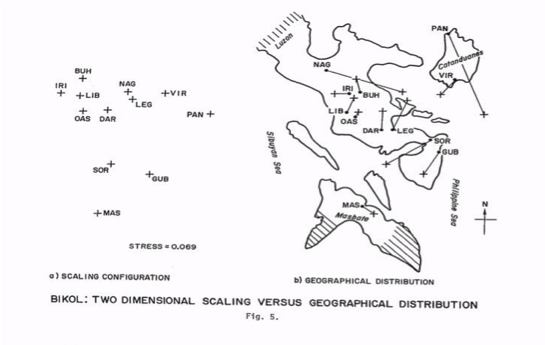
\includegraphics[scale=1]{figures/black1973.png}
    \caption{\citet{Black1973}}
    \label{fig:kaplan:black1973}
\end{figure}

On the left-hand side of Figure~\ref{fig:kaplan:black1973}, we have the distances (inverse percentage agreements) between twelve dialects scaled down to two dimensions from a potential total of eleven. The stress index given (.069) is a measure of how far these adjusted values differ from the original data fed into the program. The right-hand side shows these values projected into geographic space, with arrows indicating differences between scaled values and places where the dialects were actually observed.

This last point highlights the extent to which representational validity was of concern to those working with \textsc{mds}. The iterative nature of this method -- tinkering with dimensions and scaling to preserve fidelity to the data -- foregrounded the issue of realism in a way that pre-computational diagramming did not. If earlier examples primarily served rhetorical, didactic, or programmatic functions, \textsc{mds} thus can be seen to align with the advent of a new period of experimental visualization in comparative-historical linguistics.

In this respect, \textsc{mds} looks like a forerunner of the use of phylogenetic networks in linguistics \citep{Stevens2013}. Russell Gray, for instance, a self-described ``evolutionist'' and the newly appointed director of the Max Planck Institute for the Science of Human History in Jena, has zealously promoted the use of such probabilistic modelling techniques in linguistics, linking their powers of discovery to new scientific frontiers (e.g., \url{http://www.mpi.nl/events/nijmegen-lectures-2014/lecture-videos}, accessed 2 August 2018). Cheerfully labelling this work \emph{lexomics}, Gray has sought to model and test tacit assumptions about comparative-historical methods, in addition to reconstructing family trees.

\begin{figure}
    \centering
    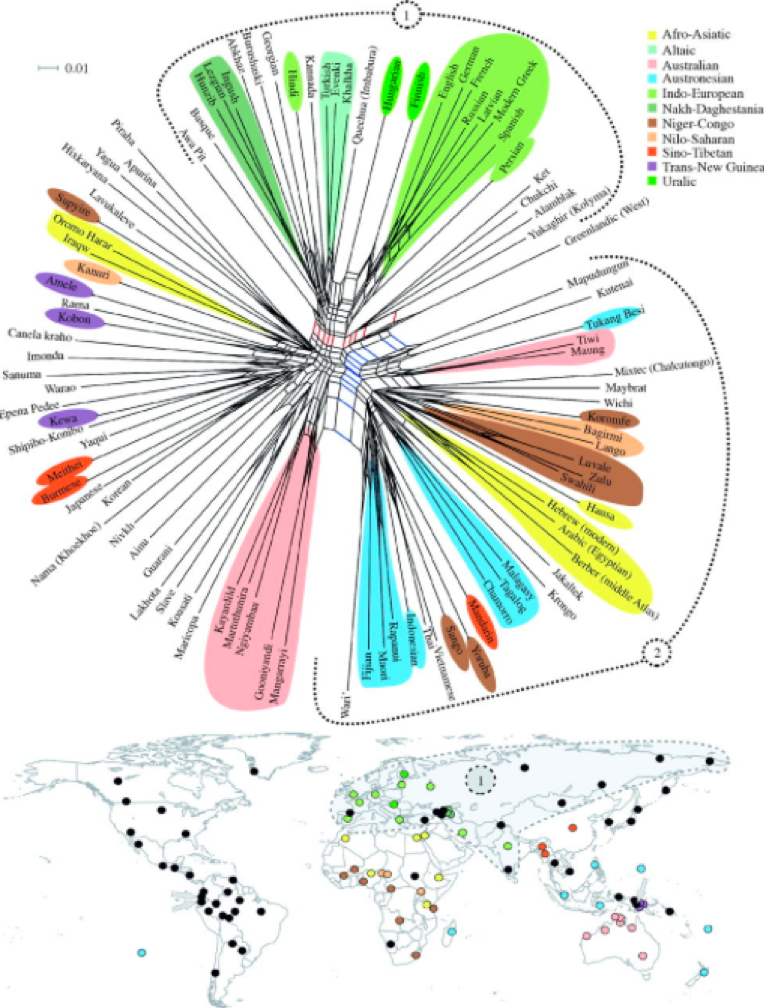
\includegraphics[scale=0.8]{figures/greenhiletal2010.png}
    \caption{\citet[2445]{Greenhilletal2010}}
    \label{fig:kaplan:greenhill2010}
\end{figure}

One of the programs commonly used in such work is SplitsTree, a tool for producing visualizations of phylogenetic networks \citep{Greenhilletal2010}. The idea, according to architects Daniel Huson (a specialist in bioinformatics at Tübingen University) and David Bryant (a mathematician from the University of Auckland) is to ``use split networks, which are not trees, to represent phylogenetic signals that, for the most part, originate from trees'' \citep[254--267]{HusonBryant2006}. Through an iterative modelling process, this program prioritizes fidelity to the givens -- acknowledging the realistic complexity of historical relationship while revealing the presence of latent trees to ``plain sight''.

\section{Conclusion}
\label{sec:kaplan:conc}

This paper has surveyed visual metaphors and visual aids of language relationship and divergence from the mid-nineteenth century to the early 2000s. It has shown that, until recently, visual metaphors took priority over visual aids. In some cases -- Schmidt's most notably -- we have seen the very utility of visual aids called fundamentally into question. The complicated overlay of mental images and concepts in this history suggests that there may be movement between these categories of metaphoric expression, accounting for both disciplinary consolidation and the open-endedness of linguistic practices. This emphasis on metaphor provides an interesting counterpoint to the recent material turn in STS scholarship on practices of scientific representation. Highlighting the difficulties linguists have encountered in their efforts to comprehend the ``all-at-once-ness'' of language relationship in both time and space, I have suggested that canonical visualizations (whether presented in words or pictures) matter a great deal in pedagogy and practice. Phylogenetic modelling has offered new hope to those in pursuit of a ``natural classification'' insofar as it offers this kind of dual vision.

\sloppy
\printbibliography[heading=subbibliography,notkeyword=this]

\end{document}
